% vim: set foldmethod=marker foldlevel=0:

\documentclass[a4paper]{article}
\usepackage[UKenglish]{babel}

% NOTE: hyperref has to come before preamble
\usepackage{hyperref}

\usepackage{preamble}

\usepackage{graphicx}
\graphicspath{ {./imgs/} }

\fancyhead[L]{MA144 Assignment 4}
\title{MA144 Methods of Mathematical Modelling 2, Assignment 4}

\begin{document}

\maketitle

\setlength{\parindent}{0em}
\setlength{\parskip}{1em}

% {{{ Q1
\question{1}

Let $C$ be the curve parametrised by \begin{align*}
x(\theta) &= (1-r) \cos \theta + r \cos \l( \f{1-r}{r} \theta \r) \\[1ex]
y(\theta) &= (1-r) \sin \theta - r \sin \l( \f{1-r}{r} \theta \r)
\end{align*}
where $r = \df1k$ and $k \in \N$. Therefore $C$ is also parametrised by \begin{align*}
x(\theta) &= \l( 1 - \f1k \r) \cos \theta + \f1k \cos \l( (k-1) \theta \r) \\[1ex]
y(\theta) &= \l( 1 - \f1k \r) \sin \theta - \f1k \sin \l( (k-1) \theta \r)
\end{align*}

Also let $D$ be the area enclosed by $C$. We want the area of $D$, which is $\ds \iint_D \d x \d y$. Green's Theorem states that $$\iint_D \l( \pdd Qx - \pdd Py \r) \d x \d y = \int_C \l( P \d x + Q \d y \r)$$

So if we just choose $P$ and $Q$ such that $\ds \pdd Qx - \pdd Py = 1$, then we can apply Green's Theorem to simplify the double integral to a single integral.

% TODO: Finish this

% }}}

% {{{ Q2
\newquestion{2}

Let $\ul F(x, y, z) = \begin{pmatrix} y^2 \\ x \\ z \end{pmatrix}$ and let $S$ be the surface parametrised by $$\ul r(u,v) = \begin{pmatrix} u \cos v \\ u \sin v \\ 3 - u \sin v \end{pmatrix}$$
where $u \in [0,1]$ and $v \in [0, 2\pi]$.

\subsection{~}
\subsection{~}

% }}}

% {{{ Q3
\newquestion{3}

\subsection{~}

\begin{figure}[h]
	\centering
	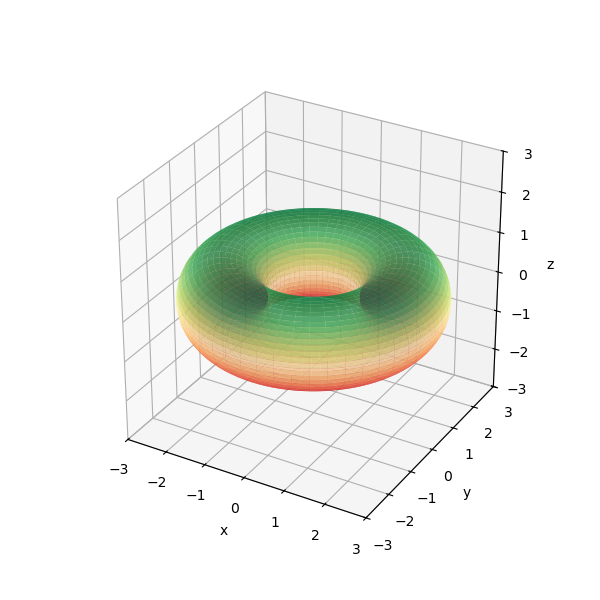
\includegraphics[scale=0.8]{Q3a-torus}
	\caption{A torus, plotted with matplotlib in Python}
	\label{fig:torus-plot}
\end{figure}

\begin{figure}[h]
	\centering
	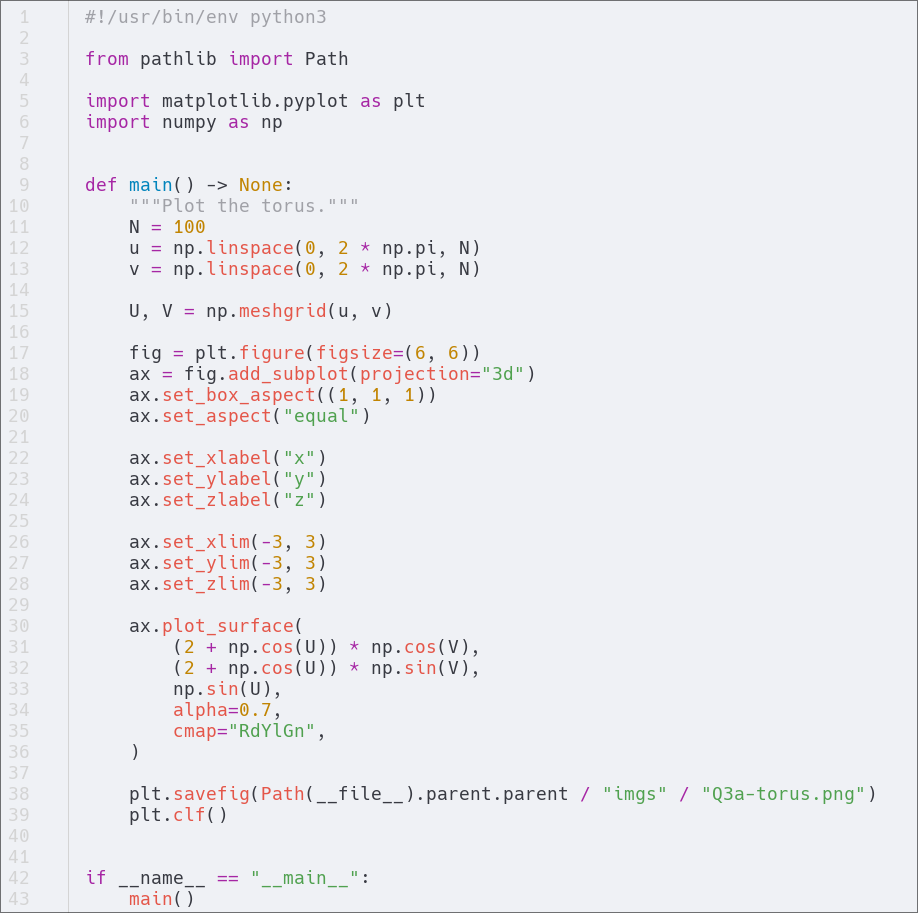
\includegraphics[scale=0.35]{Q3a-code}
	% TODO: Add proper GitHub link
	\caption{The code used to generate the plot in Figure~\ref{fig:torus-plot}. The code can also be found \href{https://github.com/DoctorDalek1963/uni}{on GitHub}}
\end{figure}

\subsection{~}

% TODO

% }}}

\end{document}
